\documentclass[a4paper]{article}
\usepackage[utf8]{inputenc}
\usepackage{textcomp}
\usepackage{geometry}
\geometry{ left=2cm, right=2cm, top=2cm, bottom=2cm, bindingoffset=5mm}
\usepackage{graphicx}
\usepackage{xcolor}
\usepackage{hyperref}
\date{}
\author{}
\usepackage{fancyhdr}
\pagestyle{fancy}
\fancyhf{}
\fancyhead[R]{2973140 - Felix Bühler \\ 2892258 - Gerhard Breul \\  3141241 - Jamie Ullerich}
\fancyhead[L]{Information Visualisation and Visual Analytics \\ WS 2019/20 }
\renewcommand{\headrulewidth}{0.5pt}
\usepackage{tikz}
\usetikzlibrary{calc}
\usepackage{amsmath}
\usepackage{cleveref}
\usepackage{subcaption}

\usepackage{changepage,titlesec}
\titleformat{\section}[block]{\bfseries}{\thesection.}{1em}{}
\titleformat{\subsection}[block]{}{\thesubsection}{1em}{}
\titleformat{\subsubsection}[block]{}{\thesubsubsection}{1em}{}
\titlespacing*{\subsection} {2em}{3.25ex plus 1ex minus .2ex}{1.5ex plus .2ex}
\titlespacing*{\subsubsection} {3em}{3.25ex plus 1ex minus .2ex}{1.5ex plus .2ex}
\setcounter{MaxMatrixCols}{20}

\title{\textbf{Assignment 10}}

\begin{document}
\maketitle 
\thispagestyle{fancy}


\section*{Task 1 - Document Similarity}
\begin{enumerate}
	\item[(a)] Sentence 1: \{impeachment: 1, -: 1, pelosi: 1, prepares: 1, to: 2, send: 1, articles: 1, senate: 1\} \\
	$(v(1) = \begin{pmatrix} 1 & 1 & 1 & 1 & 2 & 1 & 1 & 1 & 0 & 0 & 0 & 0 & 0 & 0 & 0 & 0 & 0 \\ \end{pmatrix})$ \\
	Sentence 2: \{head: 1, of: 1, hr: 1, watch: 1, denied: 1, entry: 1, to: 1, hong: 1, kong: 1\} \\
	($v(2) = \begin{pmatrix} 0 & 0 & 0 & 0 & 1 & 0 & 0 & 0 & 1 & 1 & 1 & 1 & 1 & 1 & 1 & 1 & 0 \\ \end{pmatrix}$)\\
	Sentence 3: \{senate: 1, awaits: 1, articles: 1, of: 1, impeachment: 1\}\\	
	($v(3) = \begin{pmatrix} 1 & 0 & 0 & 0 & 0 & 0 & 1 & 1 & 0 & 1 & 0 & 0 & 0 & 0 & 0 & 0 & 1 \\ \end{pmatrix}$)
	\item[(b)] $s(v(1), v(2)) = \frac{2 \cdot 1}{\sqrt{11} \cdot \sqrt{9}} = \frac{2}{9.95} = 1.809$ \\ \linebreak
	$s(v(1), v(3)) = \frac{1 \cdot 1 + 1 \cdot 1 + 1 \cdot 1}{\sqrt{11} \cdot \sqrt{5}} = 4.045$ \\ \linebreak
	$s(v(2), v(3)) = \frac{1 \cdot 1}{\sqrt{9} \cdot \sqrt{5}} = 0.745$ \\ \linebreak	
	The third sentence has a higher similarity to the first one than the second one. 
	
	\item[(c)] 
	One shortcoming is that this would result in sparse vectors which still need to be stored. 
	The second disadvantage is, that this does not take the importance of words into account. 
	It weights all words the same, but stop-words or less important ones could be neglected. 	
\end{enumerate}


\section*{Task 2 - Keyword Extraction}
\subsection*{(a)}
A lot of stop words are being displayed, which are obviously present i every other article. These words do not say anything about the content.
\subsection*{(b)}
The words reflect the content of the article. So it is much better compared to (a).
\subsection*{(c)}
\begin{figure}[!ht]
	\centering
	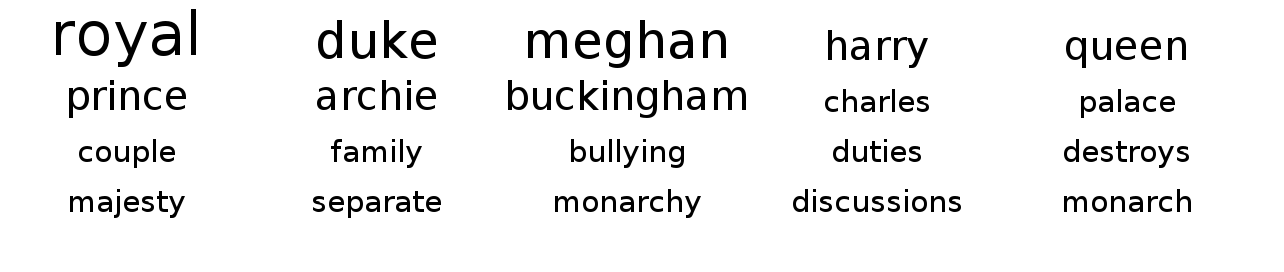
\includegraphics[width=0.7\linewidth]{ex2}
	\caption{Screenshot of Canvas}
	\label{fig:ex2}
\end{figure}


\end{document}
